\chapter{Synthesis AND Timing}
We have synthetized the architecture and we have created the report for the area and the timing.\\
\section{Area analysis}
Firstly, after the synthesis, we have retrieved the area occupied by our processor.
\begin{figure}[h!]
	\centering
	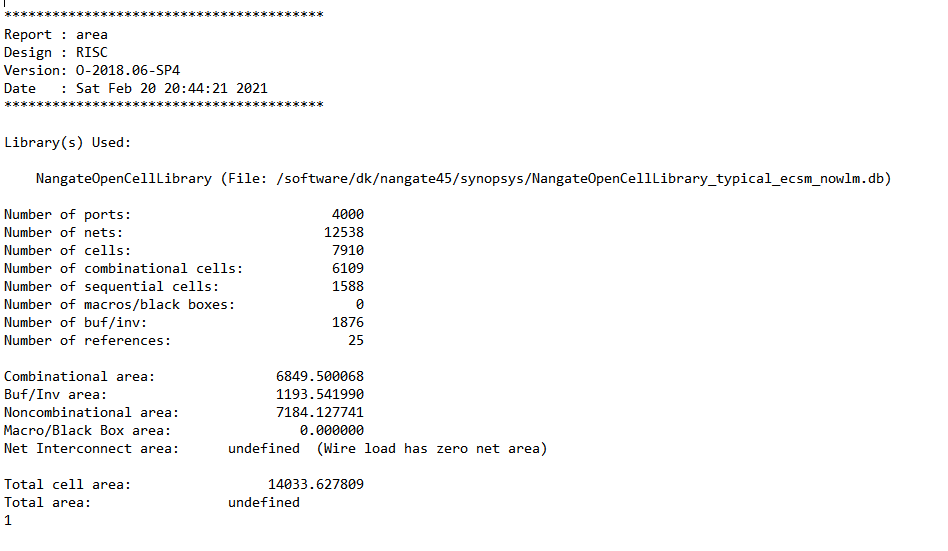
\includegraphics[width=20cm]{./images/RISC_area}
	\caption{Area report}
	\label{fig5.1}
\end{figure} 
\section{Timing analysis}
We have run the synthesis with a clock of 0s. So looking the slack,\\
we can retrieve the maximal clock frequency that our architecture can reach.
Then we have applied that contraint and we have run again the synthesis.\\
Finally we have implemented the routing phase. The result on Figure \ref{fig5.6}.
\begin{figure}[h!]
	\centering
	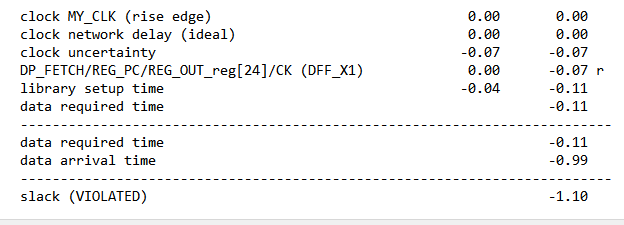
\includegraphics[width=18cm]{./images/RISC_tim0}
	\caption{Timing clock equal to 0}
	\label{fig5.2}
\end{figure}
\begin{figure}[h!]
	\centering
	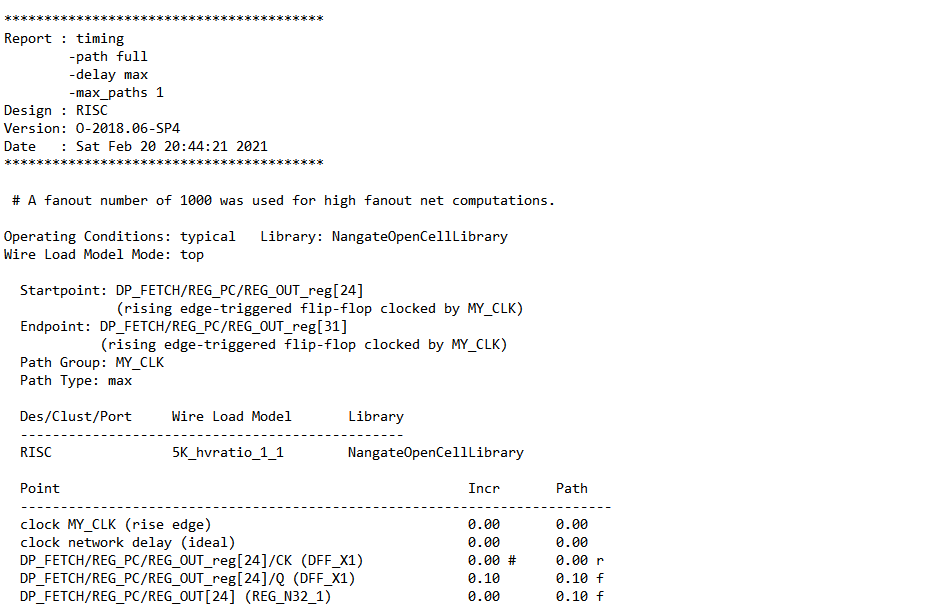
\includegraphics[width=20cm]{./images/RISC_tim1}
	\caption{Timing1}
	\label{fig5.3}
\end{figure}
\begin{figure}[h!]
	\centering
	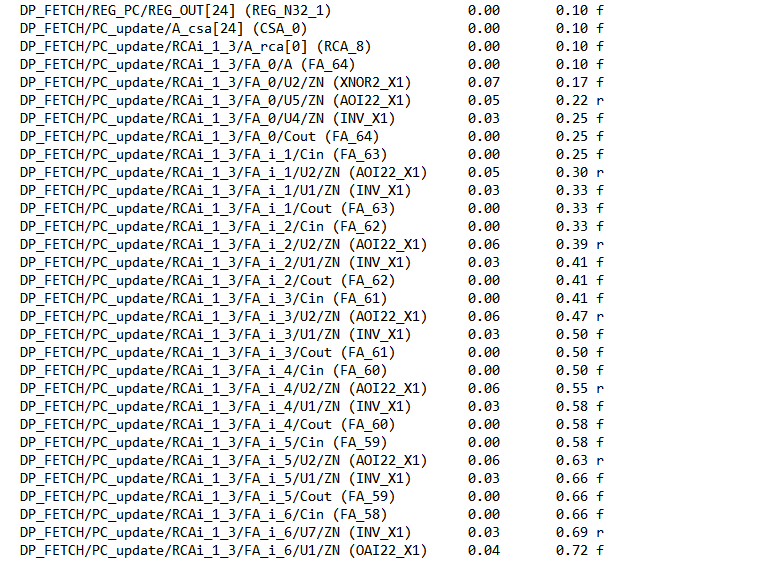
\includegraphics[width=20cm]{./images/RISC_tim2}
	\caption{Timing2}
	\label{fig5.4}
\end{figure}
\begin{figure}[h!]
	\centering
	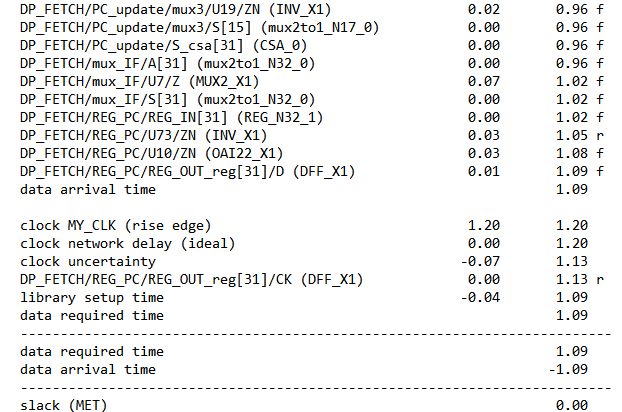
\includegraphics[width=18cm]{./images/RISC_tim3}
	\caption{Timing3}
	\label{fig5.5}
\end{figure}
\begin{figure}[h!]
	\centering
	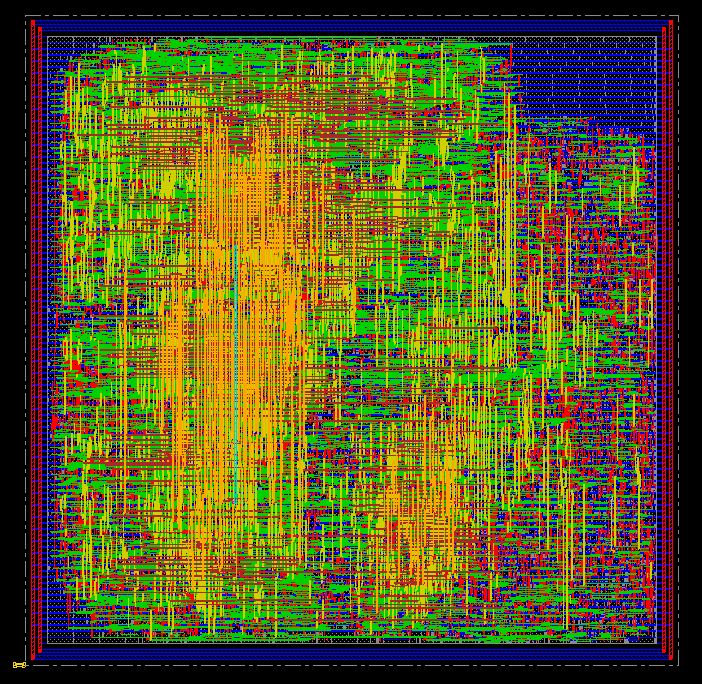
\includegraphics[width=18cm]{./images/original_route}
	\caption{Routing}
	\label{fig5.6}
\end{figure}